% -*- TeX-engine: default; -*-
\documentclass[10pt,sigconf]{acmart}
\usepackage[font=footnotesize]{subcaption}
\usepackage[utf8]{inputenc}
\usepackage[T1]{fontenc}
\usepackage{url}
\usepackage{booktabs}
\usepackage{xcolor}
\usepackage{enumitem}
\usepackage{algorithm}
\usepackage[noend]{algpseudocode}

\setcopyright{rightsretained}
\acmYear{2018}
\copyrightyear{2018}
\acmConference[CoNEXT'18]{ACM CoNEXT 2018}{December 2018}{Heraklion/Crete, Greece}

\begin{document}
\title{The eXpress Data Path: Programmable Packet Processing for the Linux Kernel}
\author{Toke Høiland-Jørgensen}
\affiliation{%
  \institution{Karlstad University}
  \country{Sweden}}
\email{toke.hoiland-jorgensen@kau.se}

\author{Jesper Dangaard Brouer}
\affiliation{%
  \institution{Red Hat}
  \country{Denmark}}
\email{brouer@redhat.com}

% \renewcommand{\shortauthors}{T. Høiland-Jørgensen et al.}
\renewcommand{\shorttitle}{The eXpress Data Path}
\captionsetup{font+=small}



\begin{abstract}
  % FIXME: Abstract should be <= 200 words
  Programmable packet processing in software has become increasingly popular, as
  increases in computational power has made it possible to run custom
  programmable pipelines at high speeds. This is generally implemented by
  so-called kernel bypass techniques, where a userspace application takes
  complete control of the networking hardware to avoid expensive context
  switches between kernel and user space.

  However, this approach makes high-speed packet processing an all-or-nothing
  proposition, where the processing application has to handle all network
  traffic, reinventing a lot of functionality already present in the kernel.
  Interoperability with other applications is also difficult, requiring
  cumbersome re-injection of packets into the kernel.

  In this paper, we present an alternative approach to programmable packet
  processing, where the kernel provides a safe execution environment for custom
  packet processing applications, executed directly in the context of the kernel
  device driver. This system, called the eXpress Data Path (XDP), is part of the
  mainline Linux kernel, and has been gradually expanded over the last several
  releases. We describe the design of the system and how it integrates with the
  rest of the kernel. Through a range of real-world examples we illustrate the
  flexibility of this model and how it can be used to implement a wide range of
  applications with performance measure in tens of millions of packets per
  second.
  % TODO: Be specific about use cases
\end{abstract}

% TODO: Add ccsxml tags and update keywords

\keywords{XDP, Programmable Networking}
\maketitle

\section{Introduction}%
\label{sec:introduction}
High-performance packet processing in software has very tight bounds on the time
spent processing each packet ($\simeq17$~ns per packet at 40 Gbps). Network
stacks in general purpose operating systems typically perform too many
operations per packet to be able to keep up with this packet rate, which has led
to increased popularity of special-purpose networking toolkits for software
packet processing, which either bypass the operating system completely, or
modify it to better accommodate high-speed packet processing. Both of these
approaches improve performance, but have the drawback that they are more
difficult to integrate with the existing networking stack, sometimes even
leading to the need to re-implement large parts of the stack. In the worst case,
this leads to the need to operate two separate stacks; one to perform high-speed
packet processing and one to run normal applications.

In this work we present an alternative approach: A novel way to integrate
programmable packet processing directly into the operating system networking
stack in a cooperative way, making it possible to perform high-speed packet
processing that integrates seamlessly with existing systems, while selective
leveraging functionality in the operating system. This framework, called the
eXpress Data Path (XDP), works by defining a limited execution environment based
on an extended version of the Berkeley Packet Filter virtual machine, which
allows verified programs to run directly in the device driver context, before
the kernel performs any other packet processing tasks.

XDP achieves extremely high packet processing performance on a single core,
making it possible to implement applications that previously required their own
appliance, such as DDOS protection and load balancing, directly on application
servers. It also allows a hybrid approach, where certain fast path processing is
offloaded to XDP while retaining normal network stack processing for other
packets. This allows for high throughput and low latency processing without
sacrificing flexibility.

While XDP has been gradually integrated into the Linux kernel over the last
several releases, no complete description of the system as a whole exists. In
this work we remedy this, and present the design of XDP, its capabilities and
integration with the rest of the Linux kernel. Our performance analysis shows
raw packet processing performance on a single core exceeding 20 million packets
per second, and scaling linearly with the number of cores. We supplement this
with three examples of real-world use cases that can be straight-forwardly
implemented in XDP:\,inline DDOS protection on a hypervisor host or application
server; load balancing by rewriting packets and resubmitting them to the
network; and a layer-3 software router implementation.

The rest of this paper is structured as follows: Section~\ref{sec:related-work}
first outlines related work. Section~\ref{sec:design} then presents the design
of XDP and Section~\ref{sec:perf-eval} presents the raw packet processing
performance analysis. Section~\ref{sec:usecases} presents the real-world use
cases and their performance. Finally, Section~\ref{sec:limitations} presents
current limitations of XDP and future work, and Section~\ref{sec:conclusion}
concludes.

\section{Related work}%
\label{sec:related-work}
\section{The design of XDP}
\label{sec:design}
XDP is designed to integrate with the Linux networking stack, enhancing it with
high-performance programmable hooks in strategic places. This makes it possible
to take advantage of the extensive and robust features of the operating system,
while adding custom packet processing as required. For this reason, XDP should
not be seen as a monolithic system one injects a single program into, but rather
a composition of individual parts that operate in concert to achieve the desired
outcome.

\begin{figure}[t]
\centering
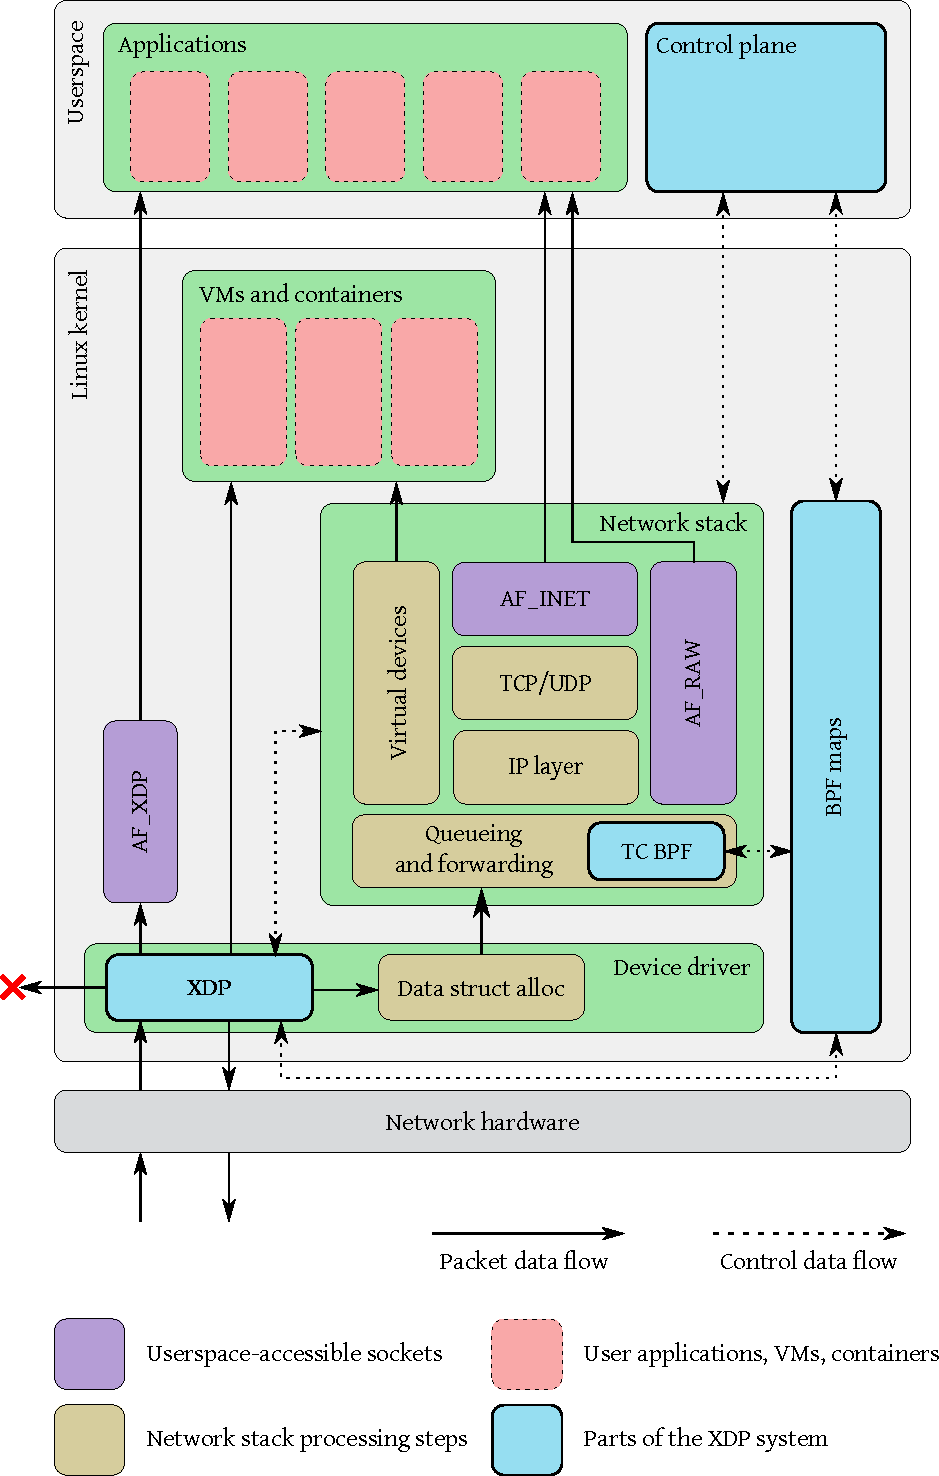
\includegraphics[width=\linewidth]{figures/kernel-diagram.pdf}
\caption{\label{fig:xdp-kernel} Diagram of how XDP integrates into the Linux
  kernel network receive path.}
\end{figure}


This section describes the various parts of the XDP system and how they fit
together. We begin with a high-level overview of the XDP programming model and
how various features of the kernel combine to form a powerful programmable data
plane. Following this, we look in detail at the extended BSD Packer Filter
(eBPF) virtual machine providing the execution model, and the in-kernel verifier
that ensures the safety of loaded eBPF programs. Finally, we give an overview of
some of the performance optimisations that are part of the XDP system, and which
help ensure high performance.

Figure~\ref{fig:xdp-kernel} shows a diagram of how XDP integrates into the Linux
kernel, and Figure~\ref{fig:xdp-execution} shows the execution flow of a typical
XDP program. Together, they give an overview of the full XDP system, and they
will be referenced throughout the exposition below.

\subsection{The XDP programming model}
\label{sec:prog-model}
The XDP system enables high-performance packet processing integrated tightly
with the rest of the Linux networking stack. This makes XDP unique compared to
other high-performance software packet processing frameworks, because it makes
it possible to selectively leverage features already implemented in Linux, while
writing custom programs to perform application-dependent processing, or to
accelerate certain parts of the data path. This section gives a conceptual
overview of the XDP programming model, explaining how the different parts fit
together.

\begin{figure*}[t]
\centering
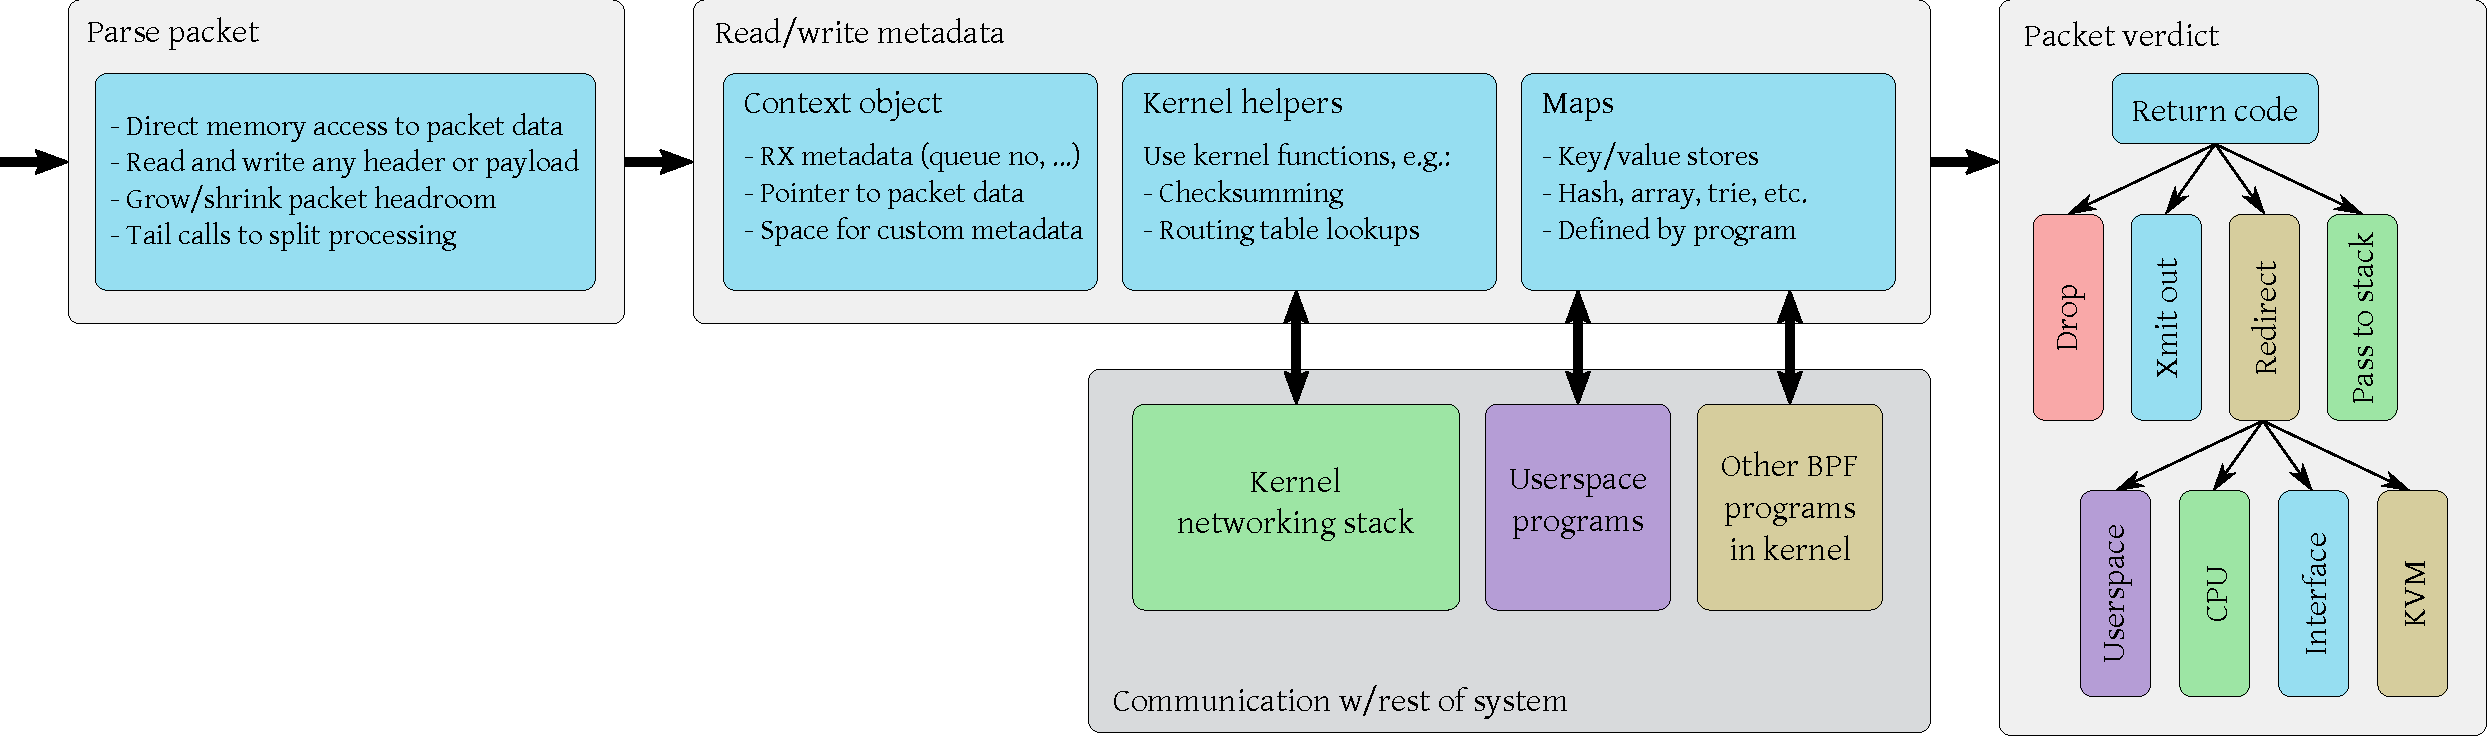
\includegraphics[width=\linewidth]{figures/xdp-execution-diagram.pdf}
\caption{\label{fig:xdp-execution} Execution diagram of a typical XDP program.
  When a packet arrives, the program starts by parsing packet headers to extract
  the information it will react on. Based on this, combined with information
  from one or more of the metadata facilities, a packet can be rewritten and a
  final verdict for the packet determined. The program can alternate between
  packet parsing, metadata lookup and rewriting, all of which are optional. The
  final verdict is given in the form of a program return code.}
\end{figure*}


An XDP program is run in the eBPF virtual machine and is entirely event driven.
The program is executed directly in context of the device driver, without
context switching to userspace. As shown in Figure~\ref{fig:xdp-kernel}, the
program is executed at the earliest possible moment after a packet is received
from the hardware, before the kernel allocates any data structures or performs
any parsing of packet data. This allows for high performance, but the program
has to parse raw packet data itself.

Figure~\ref{fig:xdp-execution} shows the various processing steps an XDP program
can perform. The program starts its execution with access to a pointer to a
context object. This object contains the buffer of the raw packet data, along
with metadata fields describing which interface and receive queue the packet
came in on, etc. The program typically begins by parsing packet data, and can
pass control to a different XDP program, through a so-called \emph{tail call},
which executes the target program and never returns to the caller, thus
splitting processing into logical sub-units (based on, say, IP header version).
The context object also contains a pointer to a special memory area is available
for XDP to store arbitrary metadata that will be available to other XDP
programs, as well as to other parts of the kernel and userspace (under certain
circumstances). The program can also write any parts of the packet data buffer,
including expanding or shrinking the packet to add or remove headers. These
three steps (reading, metadata processing, and writing packet data) correspond
to the light grey boxes on the left side of Figure~\ref{fig:xdp-execution}, and
can of course alternate and repeat in a arbitrary ways.

Similar to a regular userspace program, an XDP program ends its execution with a
return code, instructing the kernel what to do with the packet. This is shown on
the right-hand side of the figure. There are three simple return codes which
either drop the packet, immediately re-transmit it out the same network
interface, or allow the packet to be processed by the kernel networking stack.
In addition to these simple actions, the XDP program can \emph{redirect} the
packet, which controls its further processing. Redirecting can be used to
transmit the packet out a different network interface, to pass it to a different
CPU to further processing, to pass it to a virtual machine running on the host,
or to pass it directly to a special userspace socket without copying. These
different ways packets can be passed on are shown with solid lines in
Figure~\ref{fig:xdp-kernel}.

During its execution, and XDP program also has access to kernel facilities that
provide helper functions and additional metadata. These allow the XDP program to
gather additional metadata through helper functions and maps (dotted lines in
Figure~\ref{fig:xdp-kernel} and the top part of Figure~\ref{fig:xdp-execution}).
Helper functions are callbacks implemented in the kernel that an XDP program can
call to make use of kernel functionality in its processing. These helpers range
serve various purposes, ranging from simple checksum computation and hashing, to
full access to the kernel routing table. New helpers are actively been added by
the kernel development community in response to user requests, continuously
expanding the functionality that XDP programs can make use of.

Maps are key/value stores that are defined by the user before loading an XDP
program, and can be referred to from within the eBPF code. Maps are shared, both
between different eBPF programs running at various places in the kernel, as well
as between eBPF and userspace. The map types include generic hash maps, arrays
and radix trees, as well as specialised types containing pointers to eBPF
programs, or even recursive pointers to other maps. Maps serve several purposes:
they are a persistent data store between invocations of the same eBPF program; a
global coordination tool, where eBPF programs in one part of the kernel can
update state that changes the behaviour in another; and a communication
mechanism between userspace programs and the kernel eBPF programs, similar to
the communication between control plane and data plane in other programmable
package processing frameworks.

Another piece of the XDP picture is the ability to run eBPF programs in other
parts of the kernel. These include packet processing in the Traffic Control (TC)
subsystem, where eBPF programs can filter packets after they have been parsed by
the kernel, or before they are passed to the hardware from applications. This is
marked as ``TC BPF'' in Figure~\ref{fig:xdp-kernel}. In addition, eBPF programs
can be attached to various places in the kernel that are unrelated to networking
(not shown in the figures). These include \emph{cgroups}, which control resource
usage for groups of processes (used for implementing containers on Linux, for
instance), as well the \emph{tracepoint} and \emph{kprobe} introspection
subsystems which allow attaching eBPF programs to arbitrary kernel functions.
Because all eBPF programs can share the same set of maps, this makes it possible
for XDP programs to react to arbitrary events in the kernel, for instance by
dropping packets if processing load increases. Because of this integration, the
XDP programming model is considerably more powerful than just the XDP programs
itself.

A final important feature of the XDP system is the ability to dynamically load
eBPF programs. Because the kernel manages the life cycle of all eBPF programs,
they can be dynamically loaded and reloaded at runtime. Combined with dynamic
dispatch to other programs using tail calls, this makes it possible to limit the
amount of processing actually performed on packets. A processing pipeline can
simply split its processing into separate XDP programs and dynamically load and
unload them as features are enabled or disabled through control plane
configuration. This also makes it possible to dynamically compile programs with
hard-coded values derived from configuration, avoiding expensive data structure
lookups for common tasks.

The various pieces of the XDP system outlined above combine to form a powerful
programmable data plane, with integration into the Linux kernel aiding
deployment on existing systems. The following sections describe the eBPF virtual
machine itself, and the verifier that ensures that loaded programs are safe to
run in kernel space.

\subsection{The eBPF virtual machine}
\label{sec:bpf-vm}
The eBPF virtual machine is an evolution of the original BSD packet filter (BPF)
\cite{mccanne_bsd_1993} which has seen extensive use in various packet filtering
applications over the last decades. BPF uses a register-based virtual machine to
describe filtering actions. This virtual machine has two 32-bit registers and
understands 22 different instructions. This makes BPF well-suited for packet
filtering operations, but limited as a general purpose virtual machine. eBPF
extends the original BPF virtual machine to allow full general purpose execution
and efficient just-in-time (JIT) compilation into native machine code. Support
for compiling (restricted) C code into eBPF is included in the LLVM compiler
suite

The code running in the virtual machine is executed directly in the kernel
address space, which makes eBPF useful for a wide variety of tasks in the Linux
kernel. The verifier (described in the next section) ensures that user-supplied
programs cannot harm the running kernel, which enables a wide array of
integrations between the running kernel and the XDP system.

The eBPF modifies the BPF virtual machine as follows:

\begin{table}[tbp]
\caption{\label{tbl:reg-map}
eBPF to x86\_64 register mapping.}
\centering
\begin{tabular}{ll|ll|ll}
\toprule
eBPF & x86\_64 & eBPF & x86\_64 & eBPF & x86\_64\\
\midrule
R0 & rax & R4 & rcx & R8 & r14\\
R1 & rdi & R5 & r8 &  R9 & r15\\
R2 & rsi & R6 & rbx & R10 & rbp\\
R3 & rdx & R7 & r13\\
\bottomrule
\end{tabular}
\end{table}


\begin{itemize}
\item The number of registers is increased to eleven, and register widths are
increased to 64 bits, with 32-bit sub-registers accessible through certain
instructions to provide compatibility with classic BPF programs. The 64-bit
registers map one-to-one to hardware registers on all 64-bit architectures
supported by the kernel, which eases JIT compilation. For instance, the x86\_64
JIT compiler uses the mapping shown in Table \ref{tbl:reg-map}.

\item eBPF adds a \emph{call} instruction for function calls, and adopts the same calling
convention as the C language conventions used on the architectures supported
by the kernel. Along with the register mapping mentioned above, this makes it
possible to map a BPF call instruction to a single native call instruction,
enabling function calls to native kernel functions with close to zero
overhead. This facility is used by eBPF to support helpers that eBPF programs
can call to interact with the kernel while processing.

The eBPF calling convention is as follows:
\begin{itemize}
\item \texttt{R0} contains the function return value
\item \texttt{R1}-\texttt{R5} contains function arguments
\item \texttt{R6}-\texttt{R9} are callee saved registers that will be preserved across the call
\item \texttt{R10} is a read-only frame pointer to the beginning of the eBPF stack space
\end{itemize}
\end{itemize}


A BPF program starts its execution with \texttt{R1} containing a pointer to a \emph{context}
object, the contents of which varies with the type of program. For XDP, this
points to a structure that allows the BPF program to access the packet data
itself, as well as various items of metadata, including space for arbitrary data
that is carried along with the packet and is accessible by other BPF programs
that operate on the packet at later stages of processing.


\subsection{The eBPF program verifier}
\label{sec:bpf-verifier}
As mentioned in the previous section, eBPF code runs directly in the kernel
address space, which means that it theoretically has full access to the running
kernel and can either crash or compromise this. To avoid this unpleasant
situation, the kernel enforces a single entry point for loading all BPF programs
(through the \texttt{bpf()} system call). When loading a BPF program it is first
analysed by the in-kernel \emph{BPF verifier}, which ensures that the program
performs no actions that are unsafe (such as reading arbitrary memory), and that
the program will terminate by disallowing loops and limiting the maximum program
size. The verifier works by first building a directed acyclic graph (DAG) of the
control flow of the program. This DAG is then verified as follows:

\begin{table}[tbp]
\caption{\label{tbl:vrf-state-vars}
eBPF verifier state variables}
\centering
\begin{tabular}{ll}
\toprule
Variable & Contains\\
\midrule
\texttt{type} & One of the types in Table \ref{tbl:reg-types}\\
\texttt{id} & ID for tracking copies of same variable\\
\texttt{fixed\_offset} & Pointer offset (after arithmetic)\\
\texttt{range\_unsigned} & Min and max values (unsigned)\\
\texttt{range\_signed} & Min and max values (signed)\\
\texttt{tnum} & Mask and value of known bits\\
\bottomrule
\end{tabular}
\end{table}

First, the verifier performs a depth-first search on the DAG to ensure it
contains no loops (no backwards jumps) and that it contains no unsupported or
unreachable instructions. Then, in a second pass, the verifier walks all
possible paths of the DAG while tracking the state of all registers. The purpose
of this second pass is to ensure that the program performs only safe memory
accesses, and that any helper functions are called with the right argument
types. This is ensured by rejecting programs that perform load or call
instructions with invalid arguments. Argument validity is determined by tracking
the state of all registers and stack variables through the execution of the
program, as explained in the following.

\subsubsection{Register state tracking}
\label{sec:reg-state}
To track data access, the verifier assigns five state variables to each
register, listed in Table \ref{tbl:vrf-state-vars}, with the possible types listed in
Table \ref{tbl:reg-types}. The fixed offset is used to track the result of pointer
arithmetic with fixed values, while the ranges and \emph{tnum} are used to track
variable offsets of pointers, as well as the ranges of scalar variables.

\begin{table}[tbp]
\caption{\label{tbl:reg-types}
eBPF verifier type annotations. The last column indicates whether pointer arithmetic is allowed for this type of pointer.}
\centering
\begin{tabular}{lll}
\toprule
\multicolumn{3}{c}{\textbf{Non-pointer types}} \\
Name & Meaning \\
\midrule
\texttt{NOT\_INIT}            & Not initialised         \\
\texttt{SCALAR\_VALUE}        & Any numerical value       \\
\midrule
\multicolumn{3}{c}{\textbf{Pointer types}} \\
Name & Pointing to & Arithm\\
\midrule
\texttt{CTX}                  & Context              & Yes \\
\texttt{MAP}                  & BPF map              & No  \\
\texttt{MAP\_VALUE}           & Value in map         & Yes \\
\texttt{MAP\_VALUE\_OR\_NULL} & Value in map or NULL & No  \\
\texttt{STACK}                & Stack frame          & Yes \\
\texttt{PACKET}               & Packet data start    & Yes \\
\texttt{PACKET\_END}          & Packet data end      & No  \\
\bottomrule
\end{tabular}
\end{table}

At the beginning of the program, \texttt{R1} contains a pointer to the execution
context, and its type is a \texttt{CTX} pointer; \texttt{R10} is a \texttt{STACK}
pointer, and all other registers are \texttt{NOT\_INIT}. At each execution step,
register states are updated based on the operations performed by the program.
When a new value is stored to a register, it inherits the state variables of the
source of the value. Arithmetic operations on scalar values will affect the
value of the \emph{tnum} state variable, which tracks which bits in a register
are known, and their value. The \emph{tnum} is a pair of \emph{mask}, which
contains the bits whose value is unknown, and a \emph{value} which contains the
bits that are known to be set to 1. Load operations set these, for instance
loading a byte from memory will result in the top 56 bits being known to be
zero, and the bottom 8 bits to be unknown. Arithmetic updates these values
according to their operation.

Branches in the instruction tree will update the register state according to the
logical operation contained in the branch. For example, a comparison "\texttt{R1
  > 10}" compare will set the maximum value of \texttt{R1} to 10 in one branch,
and the minimum value to 11 in the other. If a comparison is performed with a
scalar value rather than a constant, the knowledge of which bits are set is used
to compute the ranges for the branches (using the minimum and maximum possible
values of unknown bits as appropriate). Finally, a branch that checks whether
register with a \texttt{MAP\_VALUE\_OR\_NULL} pointer is different from
\texttt{NULL} will turn that register into a pointer with type
\texttt{MAP\_VALUE} in the \emph{true} branch, which makes it possible to
derefence the pointer.

Using the information contained in the state variables, it is possible for the
verifier to predict the ranges of memory that it is possible for each load
instruction to access. It uses this information to ensure that only safe memory
accesses are performed. For pointers to context objects, the execution context
of the eBPF program indicates allowed memory offsets for their context objects
through a callback performed by the verifier. For map values, the map definition
defines the size of the values, which is used to bound the allowed memory
accesses. For pointers to stack values, only ranges previously stored on the
stack are valid. And finally, for pointers to packet data, only ranges known to
be less than the packet length (by appropriate compares against the packet end
pointer) are allowed. Any eBPF program that makes memory accesses that the
verifier cannot prove are safe are simply rejected at load time. The verifier
also uses the range information to enforce aligned memory accesses.

When pointers are copied to other registers, a bounds check on one copy can be
used to infer the valid ranges of the other copies, even after the copy
occurred. The \emph{id} state variable is used for this purpose for packet access and
map value pointers. For packet access, all pointers with the same variable
range will have the same \emph{id}, even if their fixed offset differs. Thus, a range
check on one copy will mark the same range (minus any differences in fixed
offsets) as valid in the other copies. Similarly, for pointers to map values,
all copies of a pointer returned from the same map lookup share their \emph{id}, and
a check against NULL will be valid for all of them.



\subsection{Performance Optimisations in XDP}
\label{sec:perf-optim-xdp}

Much of the performance improvement that XDP represents over the standard Linux
networking stack is due to the processing happening before data structures are
created and memory allocated. However, there are also a couple of performance
enhancement techniques that have specifically been applied over the development
of XDP (although some of them also benefit the normal stack). In this section we
outline these techniques, and how they apply to XDP.

Packet processing on general-purpose hardware, as is done with XDP, inevitably
carries some overhead costs related to getting the packets transferred to the
system memory, processing them by the CPU, and sending them back to the
hardware. Amortising these costs over multiple packets through bulking is an
essential technique to achieve high performance. In Linux, there are two main
ways bulking is achieved: On the receive path, the NAPI mechanism~\cite{napi}
amortises the cost of interrupts from the hardware, by temporarily turning off
interrupts each time a packet is received, and instead polling to receive a
batch of packets at once. This mechanism has been available in Linux for a long
time; but for XDP it carries with it additional benefits, since the XDP program
can be executed directly in the NAPI poll context.

A similar issue is seen on the transmit path, where updating the tail pointer in
the device ring buffer initiates a transmit operation to the hardware, which
carries with it some overhead. To amortise this, XDP uses two mechanisms: When
the XDP program indicates that the packet should be transmitted out on the same
interface it came in on, it is put into the transmit ring buffer immediately,
but the tail pointer update is deferred until the end of the NAPI poll sequence,
which causes batching of all packets in the same sequence on transmit as well.
When redirecting packets to a different interface, another mechanism is used to
achieve the same thing: the redirect mechanism can use a BPF map to lookup the
destination interface. When doing so, the map also contains a buffer that will
be used to batch packets from subsequent calls, and defer the actual
transmission out of the destination interface until the end of the NAPI poll
sequence. Using the map structure to achieve this makes it transparent to the
calling program and even the device driver.

\section{Performance evaluation}
\label{sec:perf-eval}
In this section we present our performance evaluation of XDP, using synthetic
benchmarks to look at specific aspects of the packet processing capabilities. In
the next section, we supplement this with a description and evaluation of a
series of real-world use cases.

For all benchmarks, we use a machine equipped with a hexa-core Intel Xeon
E5-1650 v4 CPU running at 3.60GHz, and memory modules installed in all four
memory slots, to get the full available memory bandwidth. This CPU supports
Intel's Data Direct I/O (DDIO) technology, which makes it possible for the
networking hardware using Direct Memory Access (DMA) to place data directly into
the processor cache, which eliminates cache misses on subsequent processing of
the data. The test machine is equipped with two Mellanox ConnectX-5 dual-port
100Gbps network adapters, installed in PCI Express v3 16-lane slots, which
ensures that the PCI bus has enough nominal bandwidth available to match the
network adapter speed for a single port on each card. However, even so, in some
of our tests the performance is bottlenecked at the PCI bus, as we will see
below.

We use the TRex packet generator~\cite{cisco18:_trex_traff_gener} to produce the
test traffic. The test machine runs a version of the Linux kernel that will
be released as v4.18. We make details of our setup, links to source code and the
raw test data available in an online repository~\cite{test-data}.

To show the performance achievable with XDP, we perform the following
measurements, which correspond to the four different return codes shown in
Figure~\ref{fig:xdp-execution} above:

\begin{itemize}
\item Packet drop performance. We install a simple XDP program that drops
  packets after receiving them, to examine the maximum possible packet
  processing performance.

\item Packet mirroring performance. Here we measure the performance of sending
  packets out the same network interface that they arrived on.

\item Packet forwarding performance. Here we install a simple XDP program that
  redirects packets out a different interface as they arrive.

\item Inline packet processing. We install an XDP program that allows the
  packets to proceed to the kernel networking stack, to measure the overhead
  that XDP processing introduces in the kernel receive path.
\end{itemize}


For all of these tests, we measure the maximum how many packets per second the
system can process, as well as the CPU usage required for processing different
offered loads. We compare the performance with the \texttt{testpmd} example
application shipped with DPDK framework, and with the regular Linux kernel
network stack (except for the inline processing use case, which is specific to
XDP). For all tests, we use minimum-sized (64 bytes) packets, since processing a
high number of packets per second is the most challenging, and using larger
packets only exacerbates the PCI bus bottleneck.

\subsection{Packet Drop Performance}
\label{sec:basel-pack-proc}
Figure~\ref{fig:drop-test} shows the packet processing performance as a function
of the number of cores. The baseline performance of XDP for a single core is
26\,Mpps, while for DPDK it is 43.5\,Mpps. This scales linearly with the number
of cores, until it hits the maximum capacity of our traffic generator, at
82.5\,Mpps. DPDK reaches this with 3 cores, while for XDP it takes 4. However,
we believe it is likely that both XDP and DPDK would be able to continue scaling
beyond these limits given a suitable traffic source. \textbf{FIXME: Is this
  true?}

\begin{figure}[t]
\centering
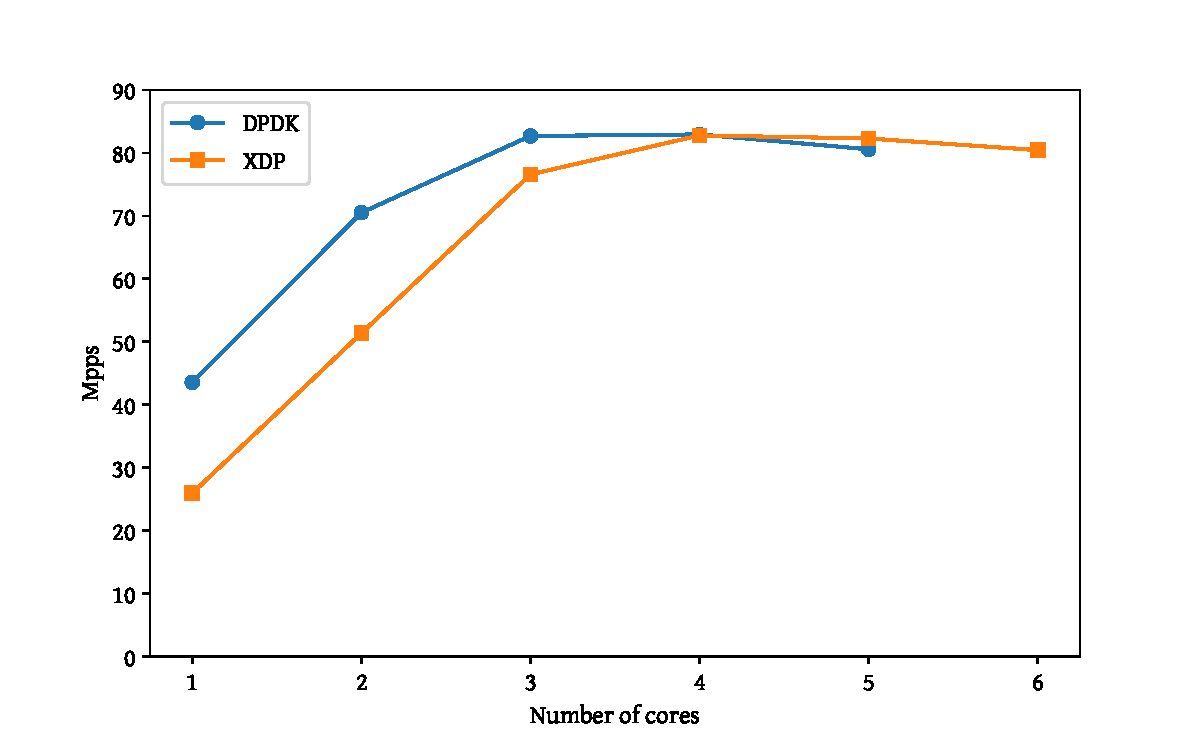
\includegraphics[width=\linewidth]{figures/drop-test.pdf}
\caption{\label{fig:drop-test} Packet drop performance. DPDK uses one core for
  control tasks, which is why it only goes to 5. The slight downward trend at
  above 4 cores is because the performance of our packet generator decreases
  when it has to generate more streams.}
\end{figure}


The reason the performance dips at five and six cores is because dividing the
traffic over several cores requires using the Receive Side Scaling (RSS)
features of the hardware, which can divide up traffic between hardware receive
queues (each of which is bound to a separate core) based on packet header
information. Using this requires the traffic generator to generate the traffic
as separate flows, which means its maximum throughput drops.

\subsection{Packet Mirroring Performance}
\label{sec:pack-mirr-perf}

TBD. FIXME: Can we do this with DPDK?

\subsection{Packet Forwarding Performance}
\label{sec:pack-forw-perf}
Figure~\ref{fig:redirect-test} shows the packet forwarding performance. Again,
we see an almost linear scaling with the first couple of cores, tapering off to
sub-linear performance increases as more cores are added. We attribute this to
\textbf{FIXME}.


\begin{figure}[t]
\centering
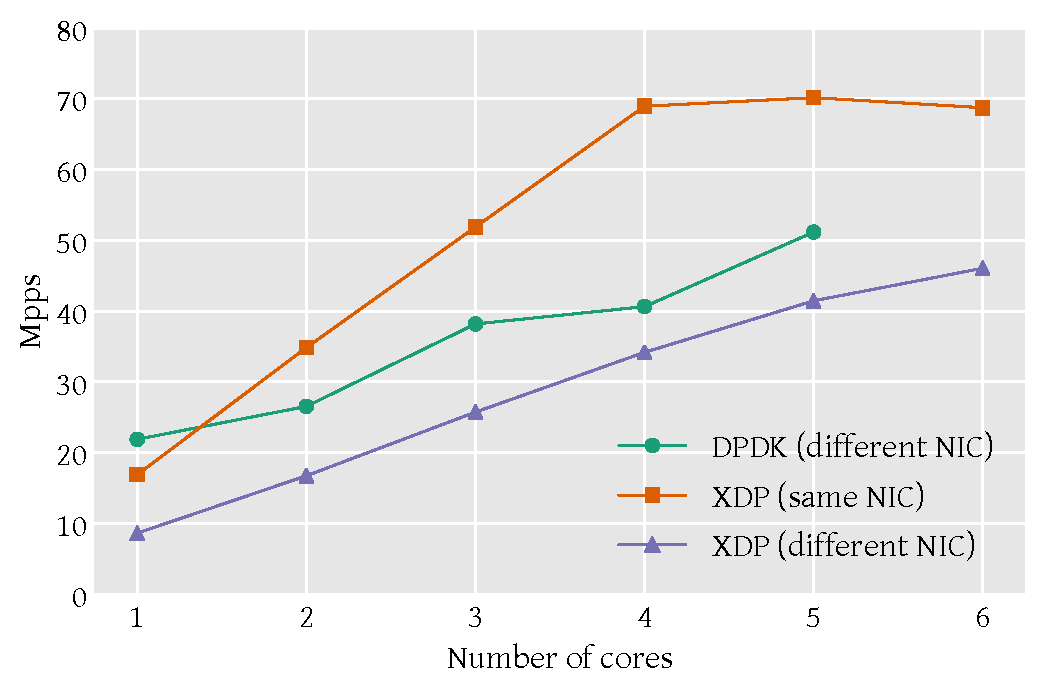
\includegraphics[width=\linewidth]{figures/redirect-test.pdf}
\caption{\label{fig:redirect-test} Packet forwarding performance.}
\end{figure}

\section{Real-world use cases}
\label{sec:usecases}
In this section we describe and evaluate three real-world use cases that
showcase various ways in which XDP can used to implement useful applications or
features. These use cases have all seen real-world deployment in one form or
another, although we use simplified versions in our evaluation so as to be able
to make the code available.

The three use cases are inline Denial of Service (DoS) mitigation, a software
layer-3 router, and an application load-balancer, and are described in turn in
each of the following subsections.

\subsection{Inline DoS Mitigation}
\label{sec:dos-usecase}
DoS attacks continue to plague the internet, typically in the form of
distributed attacks (DDoS attacks) from compromised devices attached to the
internet. There are various ways to mitigate them, but having some kind of
service that protects critical infrastructure is typically at least a component
of DDoS mitigation \textbf{FIXME: citation needed}. This can be done by
filtering all traffic through a device that distinguish legitimate traffic from
attacks, and drop the attack packets before they reach the application server.

The obvious problem with protecting against a DDoS attack is the sheer scale of
the traffic that needs to be dropped, which leads to the use of expensive
appliances to handle the dropping. However, with XDP we have another option:
installing the traffic filter directly on the application server in the form of
an XDP program, which is possible without any other modifications to the server.
In the case of a virtual machine deployment, the filter can even be installed on
the hypervisor, and thus protect all virtual machines running on the host.

How to identify attack traffic is not our focus here, but rather the mechanism
that drops the unwanted traffic. We simply assume that there exists \emph{some}
way of identifying which traffic is legitimate and which isn't. Because of the
dynamic nature of XDP, there are many options available: BPF maps could be used
for while-listing or black-listing, the packet payload could be inspected, etc.
It is even possible to load new XDP programs especially tailored towards
dropping a particular kind of attack traffic as the need arises. However, in our
example, we simply assume that a server hosts a TCP-based service, and so
consider all UDP traffic as unwanted.

To test the performance of such a solution, we use the Netperf benchmarking
tool~\cite{netperf}. This is equipped with a TCP-based round-trip benchmark,
which opens a TCP connection and sends a small payload which is echoed back from
the server, repeating as soon as a reply is received. The output is the number
of transactions per second, which is a good proxy for an interactive TCP
session, such as small remote procedure calls.

We first measure the baseline performance of this test, and see that we are able
to perform around 25.000 transactions per second with no competing traffic. We
then, from a separate machine, offer an increasing load of small UDP packets,
which simulates the DoS attack, and measure how the TCP application is affected.
The network interface is configured to redirect all traffic to a single receive
queue, so all packets are processed by the same CPU core. This is important in
this use case, because the machine will be running other applications on the
remaining cores, and so we don't want to dedicate too many resources to just
packet processing\footnote{The actual number of cores dedicated to packet
  processing will of course have to depend on the volume of traffic the filter
  should be able to process.}.

\begin{figure}[t]
\centering
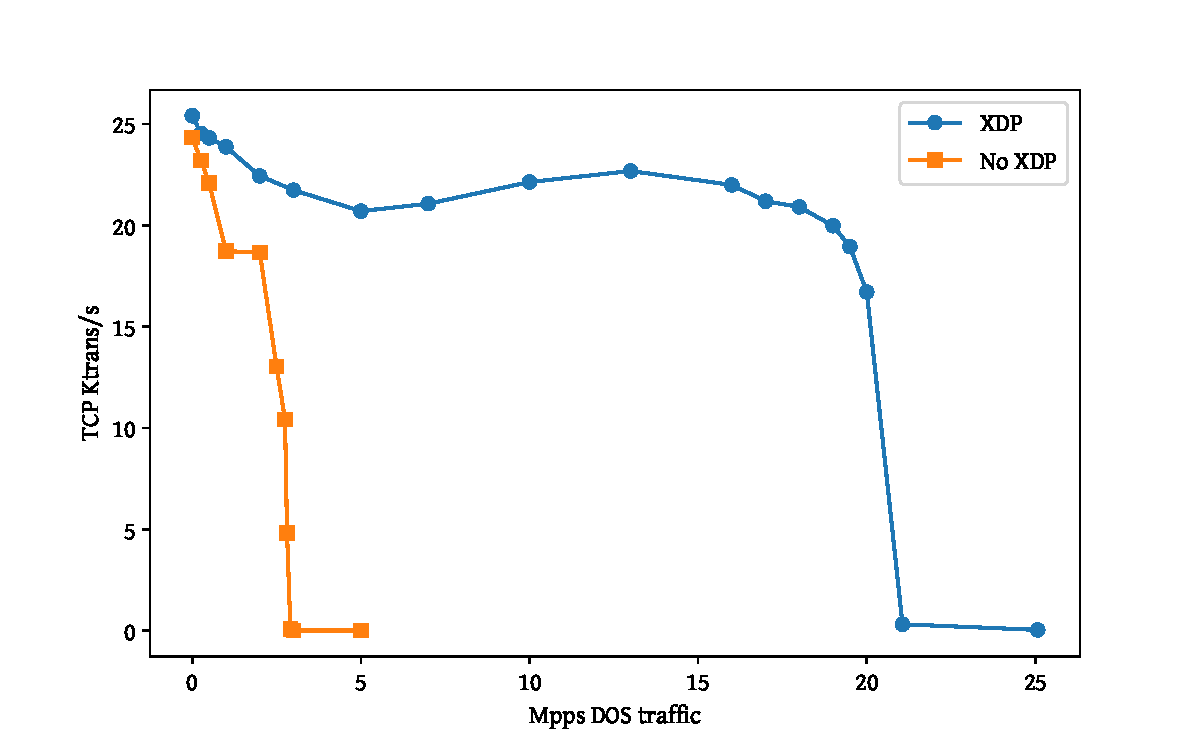
\includegraphics[width=\linewidth]{figures/ddos-test.pdf}
\caption{\label{fig:ddos-results} DDOS performance. Number of TCP transactions
  per second with different levels of UDP packet floods being sent to the
  server.}
\end{figure}

The results of this is shown in Figure~\ref{fig:ddos-results}. It is clearly
seen that without the XDP filter, performance drops significantly, being halved
at 2.5 Mpps and effectively zero at just below 3 Mpps. However, with the XDP
filter in place, performance is kept above 20.000 transactions per second up to
19 Mpps, after which it drops rapidly. The small increase in baseline
performance (from 24,500 to 25,500 transactions per second) is because the XDP
program uses the \emph{redirect} feature to move the network stack processing of
the application traffic to a separate CPU core, to make sure the application
performance is not impacted by handling of the DoS traffic.

As these results show, it is quite feasible to perform this kind of filtering in
XDP, and comfortably handle packet rates above 10\,Gbps of DoS traffic (with
minimum packet sizes) on a single CPU core. Deploying DoS mitigation this way
leads to increased flexibility, both because of the programmability offered by
XDP, but also because it eliminates the need for at separate appliance to scrub
the traffic.

\subsection{Software Router}
\label{sec:fwd-usecase}
The second use case is that of a software router. The Linux kernel already
contains a full-featured routing table, which includes support for policy
routing, source-specific routing, equal-cost multipath load balancing, and more.
And routing daemons such as Bird or FRR implement a variety of routing control
plane protocols, which makes it quite feasible to turn a Linux system into a
full-featured software router. However, thus far the data plane forwarding
performance has kept this from being feasible at very high rates.

Because of the rich ecosystem for routing on Linux, improving performance of the
kernel data plane is desirable, as re-implementing the routing stack in another
data processing framework carries a high cost. Thus, XDP is particularly suited
for this task. This is also the reason why one of the first kernel helpers
introduced to XDP is a routing table lookup function. This function makes it
possible to perform full routing table lookups directly from XDP. The result of
the lookup is an egress interface and a next-hop MAC address, which makes it
possible for the XDP program to immediately forward the packet if the lookup
succeeds. If no next-hop MAC is known (because neighbour lookup hasn't been
performed yet), the XDP program can instead pass the packet to the networking
stack, which will perform the neighbour lookup, allowing subsequent packets to
be forwarded by the XDP fast path.

To show the performance of the software router use case, we use the XDP routing
example that is included in the Linux kernel source and compare its performance
to the native Linux networking stack routing. The example simply parses the IP
header of an incoming packet, does a routing table lookup, and immediately
forwards the packet if a match is found, or passes it up to the network stack if
not. We perform two tests: one with a single route installed in the routing
table and all packets set to the same destination address. And another where we
import a full dump of the global BGP routing table from \url{routeviews.org},
where we set all next-hop addresses to the same value, but vary the source
addresses of the packets being routed. In the first test we compare the
performance with the layer-3 forwarding example included with the DPDK source
code; but because this example only supports a fixed routing table, we do not
perform the full BGP table comparison with DPDK.

The performance of this use case is seen in Figure~\textbf{FIXME}.

\subsection{Load-balancer}
\label{sec:org685e28c}
\begin{itemize}
\item \texttt{XDP\_TX}
\item \texttt{XDP\_REDIRECT} to CPU/VM
\end{itemize}

\section{Limitations and future work}
\label{sec:limitations}


\section{Conclusions}
\label{sec:conclusion}





\bibliographystyle{ACM-Reference-Format}
\bibliography{xdp}

\end{document}
